\documentclass[12pt,a4paper]{article}
% \usepackage[UTF8]{ctex}
\usepackage{fontspec}
\usepackage{titletoc}
\usepackage{xeCJK}
\usepackage{graphicx}
\usepackage{amsmath}
\usepackage{indentfirst} % 中文首段缩进
\usepackage{minted} % 代码块高亮渲染

\setmainfont[Path=/usr/share/fonts/wenquanyi/wqy-microhei/]{wqy-microhei.ttc}
\setCJKmainfont[Path=/usr/share/fonts/wenquanyi/wqy-microhei/]{wqy-microhei.ttc}
% \setmainfont[Path=/mnt/data/Fonts/NotoSans/]{NotoSans-Regular.ttf}
% \setCJKmainfont[Path=/mnt/data/Fonts/NotoSans/]{NotoSans-Regular.ttf}

% 图片位置
\graphicspath{ {img/} }

\usepackage{xcolor}
\usepackage{hyperref}
\hypersetup{
    colorlinks=true,
    linkcolor=blue,
    urlcolor=cyan,
    linktoc=all,
	pdftitle={RSA和DES加密实验},
	bookmarks=true
}

% 行内代码背景颜色和相关快捷命令
\definecolor{bg}{rgb}{0.95,0.95,0.95}
\newmintinline[incode]{text}{bgcolor=bg,breaklines,breakanywhere}
% \newcommand{\incode}[1]{\begin{verbatim}#1\end{verbatim}} % 定义行内代码渲染命令
% \newcommand{\codefile}[1]{\inputminted[bgcolor=bg,linenos,tabsize=4]{verilog}{code/#1}} % 定义行内代码渲染命令
	
\renewcommand{\baselinestretch}{1.1} % 定义行间距
\parindent 24pt % 重新定义缩进长度
 
%%%%%%%%%%%%%%%%%%%%%%%%%%%%%%%%%%%%%%%%%%%%%%%%%%%%%%%%%%%%%%%%
%  lengths
%    下面的命令重定义页面边距,使其符合中文刊物习惯。
%%%%%%%%%%%%%%%%%%%%%%%%%%%%%%%%%%%%%%%%%%%%%%%%%%%%%%%%%%%%%%%%
\addtolength{\topmargin}{-54pt}
\setlength{\oddsidemargin}{-0.9cm}
\setlength{\evensidemargin}{\oddsidemargin}
\setlength{\textwidth}{18.00cm}
\setlength{\textheight}{25.50cm}    % 24.62

% 标题、作者、日期等信息
\title{RSA和DES加密实验}
\author{张海斌\thanks{学号 17307130118}}
\date{2019年11月}


\begin{document}

\maketitle

% 目录
\renewcommand\contentsname{目~录} % 目录名称
\tableofcontents

\section{界面说明}

\begin{figure}[htbp]
	\centering
	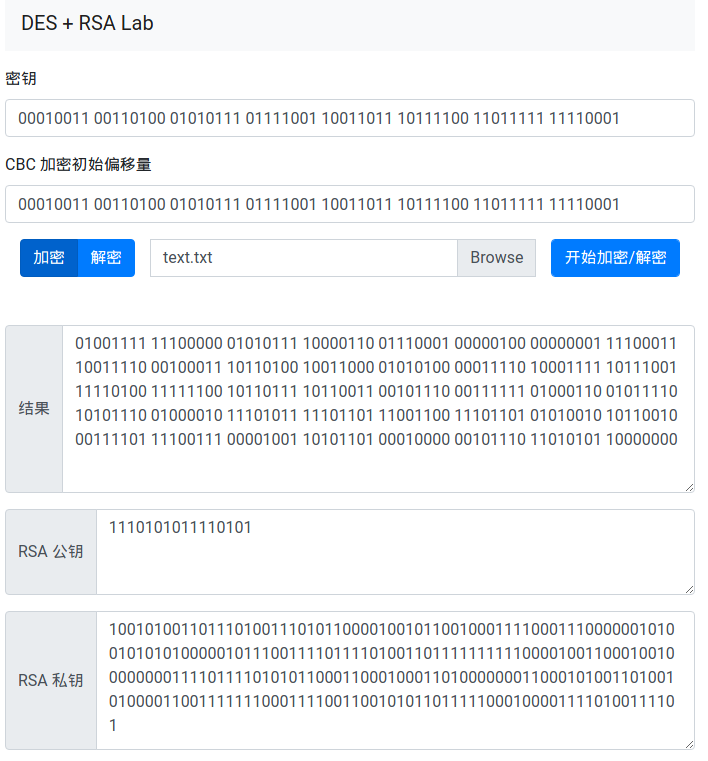
\includegraphics[width=\textwidth]{front}
	\caption{前端界面}
	\label{fig:front}
\end{figure}

如\autoref{fig:front},数据输入界面和之前的DES实验的前端界面一致。手动输入DES密钥、和初始偏移量,并选择加解密方法和要加密的文件,最后点击"开始加密/解密"按钮即可加密。不同之处在于结果显示多了很多RSA的加解密的结果,如\autoref{fig:rsa}:\incode{RSA公钥}、\incode{RSA私钥}分别用于对DES密钥进行加密得到密文,和将密文解密得到原始的DES密钥。还有\incode{RSA n}表示RSA取模的大小,以及\incode{RSA加密}和\incode{RSA解密}分别对应用RSA加密DES密钥和解密RSA密文得到的结果。

在访问该前端网页的时候,会自动获取新的随机密钥对并显示在界面上。提交DES加/解密操作之后会显示出DES加解密的结果,同时也会显示出RSA对DES密钥进行加解密的结果。操作成功提示界面也略有更改,如\autoref{fig:result}。

运行环境需要Python和Flask。执行\incode{run.bat}或\incode{run.sh}脚本即可运行。示例输入数据见\incode{example}文件夹里。\incode{text.txt}为明文,\incode{key.txt}为DES密钥,\incode{iv.txt}是CBC加密的初始偏移量,\incode{ciphertext.txt}是DES加密后的结果,将它用通过RSA加密算法传输的DES密钥解密后的结果与\incode{text.txt}明文相同,说明DES和RSA的算法都是正确的。


\begin{figure}[htbp]
	\centering
	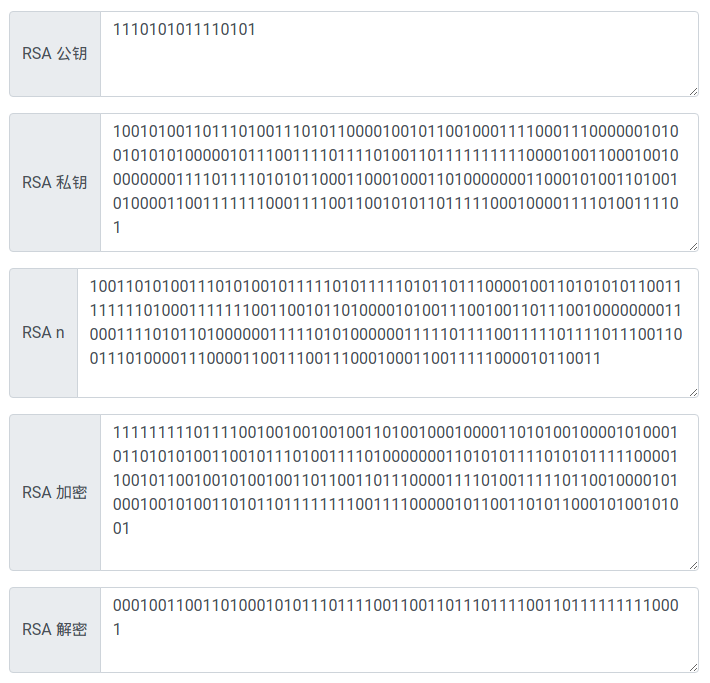
\includegraphics[width=\textwidth]{rsa}
	\caption{RSA 加解密结果}
	\label{fig:rsa}
\end{figure}

\begin{figure}[htbp]
	\centering
	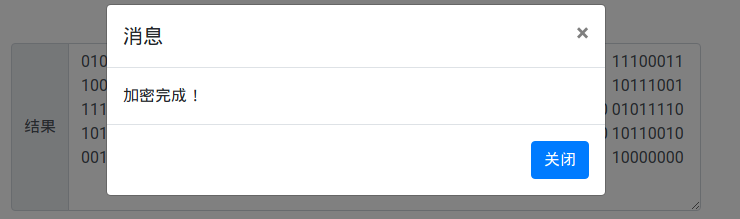
\includegraphics[width=\textwidth]{result}
	\caption{提示界面}
	\label{fig:result}
\end{figure}

\section{RSA 实现}

RSA的Python实现代码在\incode{rsa.py}文件中。主要函数功能有快速幂取模、扩展欧几里得算法、Miller-Robin检测质数、获取一个指定位数的质数。在这之上有三个用于进行RSA加解密的函数:生成密钥对的函数\incode{generateKeys}、对明密文加解密的函数\incode{encryptRSA}和\incode{decryptRSA}。

质数检测函数中使用多次Miller-Robin的方法检测质数,保证几乎可以完全确定是质数。检测次数可以通过修改变量\incode{primeTestRound}的值改变。在生成RSA密钥对时e的选取,我直接选择一个16位的质数作为e的值。

由于64位的DES密钥开头可能是0开头,导致最后RSA解密出的结果长度小于64位,所以我用0扩充RSA解密的结果到64位来避免加解密后长度不一致的问题。

\end{document}
